\documentclass[conference]{IEEEtran}
\IEEEoverridecommandlockouts
\usepackage{amsmath,amssymb}
\usepackage{booktabs}
\usepackage{graphicx}
\usepackage{xcolor}
\usepackage{pgfplots}
\pgfplotsset{compat=1.16}
\usepackage[hyphens]{url}
\usepackage{cite}

% Build: tectonic main.tex   (IEEEtran conference format, same as the earlier draft)
\begin{document}

\title{Do the Numbers Hold on Real Hardware? A Measurement-Based Re-Evaluation of a Low-Cost Hybrid ECC Authentication Protocol for IoT}

\author{\IEEEauthorblockN{Jay Kerkar, Chaitanya Kelkar, Chirag Poornamath, Yash Kolekar}
\IEEEauthorblockA{Department of Information Technology\\
Vivekanand Education Society's Institute of Technology\\
Mumbai, India}
\and
\IEEEauthorblockN{Dr.\ Shanta Sondur}
\IEEEauthorblockA{\textit{Project Guide}\\
Department of Information Technology\\
Vivekanand Education Society's Institute of Technology\\
Mumbai, India}}

\maketitle

\begin{abstract}
Al-Rasheed et al.\ proposed a two-message hybrid ECC/symmetric-key mutual-authentication protocol for the Internet of Things and reported roughly 17\%, 21\% and 12\% lower communication, processing and storage cost than prior schemes. Those figures come from OMNeT++ simulation and from assumed per-operation times, not from measurements. We (i) audit the paper's own tables and figures, (ii) implement the device side in C, interoperate it with an independent Python server on an ESP8266 microcontroller, and (iii) time the underlying primitives on the ESP8266, an AWS Graviton2 core and a laptop, then recompute the paper's cost model with measured values. The headline percentages cannot be derived from the paper's tables or figures under any definition we tried, and the tables contradict the text (four messages and 1024 bits versus two messages and 264 bits). Measured P-256 scalar multiplication on the ESP8266 takes 276~ms, sixteen times the assumed 17.1~ms, while symmetric operations are five to twelve times faster than assumed. The protocol is therefore roughly 120--3\,000$\times$ cheaper than the ECC-based schemes it is compared with, but once the session-key derivation required by its own equations is counted, it costs more than each of the three hash-only schemes in the same comparison, in every cost column, on every platform we measured, including hardware-accelerated cryptography. We also show that the scheme lacks forward secrecy, uses no elliptic-curve operation online, and that its server-side pseudonym lookup grows linearly with the number of devices. All code and raw data are open.
\end{abstract}

\begin{IEEEkeywords}
Internet of Things, mutual authentication, elliptic curve cryptography, reproducibility, microcontroller benchmarking, lightweight security.
\end{IEEEkeywords}

\section{Introduction}
Lightweight authentication schemes for the Internet of Things (IoT) are usually compared by counting cryptographic operations and multiplying by assumed per-operation times. The conclusion of such a comparison then depends on a few constants that are rarely measured on the class of device the scheme targets. Al-Rasheed et al.~\cite{base} propose a hybrid scheme in which elliptic-curve cryptography is confined to an offline registration phase and every online authentication uses a two-message nonce-based symmetric handshake. They report about 17\%, 21\% and 12\% lower communication, processing and storage cost than ten prior schemes, using OMNeT++ simulation and the reference times of their Table~III (an ECC scalar multiplication at 17.1~ms, a symmetric encryption or decryption at 5.6~ms, a SHA-1 hash at 0.32~ms).

We test those claims end to end. Our contributions are:
\begin{enumerate}
\item \textbf{A consistency audit} of the paper's tables, equations and figures (Section~\ref{sec:audit}).
\item \textbf{Measured primitive costs} on a 32-bit microcontroller (ESP8266), an AWS Graviton2 core and a laptop, using one C source on every platform with checksum-verified outputs, and a recomputation of the paper's cost model with a sensitivity analysis (Sections~\ref{sec:constants} and~\ref{sec:ranking}).
\item \textbf{Protocol-level findings} that bear on how the scheme should be compared: no forward secrecy, no online elliptic-curve operation, and a server lookup cost that grows with the number of devices (Section~\ref{sec:protocol}).
\item An \textbf{open implementation and benchmark}: a Python reference of the protocol, a portable C device core, ESP8266 firmware, and the audit scripts.
\end{enumerate}

\section{The Base Protocol and Its Evidence}
\label{sec:base}
In the offline phase a trusted authority (TA) derives a long-term secret $\lambda_X = H_1(\mathrm{ID}_X\,\|\,s) \bmod n$ for each device and server (Eq.~8 of~\cite{base}) and distributes peer secrets, so that both sides can compute a pairwise root $k^\star_{ij}=\mathrm{KDF}(\lambda_{V_i}\,\|\,\lambda_{R_j})$ (Eq.~9). Online, a device sends $M_1=\langle \mathrm{PID}_{V_i,t}, C_1,\mu_1\rangle$ with $\mathrm{PID}=H_2(\lambda_{V_i}\,\|\,t)$, $C_1=\mathrm{Enc}_{k^\star}(\mathrm{PID}\,\|\,N_i\,\|\,t)$ and a MAC $\mu_1$; the server replies with $M_2$, and both derive the session key $K=\mathrm{KDF}(k^\star\,\|\,N_i\,\|\,N_j\,\|\,t)$ (Eq.~16). The instantiation notes name AES-GCM~\cite{gcm}, HKDF~\cite{hkdf} and SHA-256. The online cost is stated as one KDF, one encryption and one MAC on the device (Eq.~22).

Cost claims rest on Tables~IV--VI, which compare the proposed scheme with schemes labelled \cite{porambage,turkanovic,dhillon,jiang,challa,sadhukhan,fakroon} and others, and on Figs.~1--3, which compare against four different schemes. Processing cost (Table~V) is a per-role count of hash ($T_H$), symmetric ($T_{SE/D}$), ECC scalar-multiplication ($T_{ECM}$) and fuzzy-extraction ($T_{fe}$) operations, multiplied by the Table~III constants.

\section{Methodology}
\label{sec:method}
\subsection{Audit}
Tables~III--VI were transcribed from 300-DPI renders of the published PDF and re-read at 600~DPI. Tables~III, IV and VI were additionally checked by optical character recognition (every cell matched); Table~V, whose mathematical typography defeats OCR, was checked by two manual cell-by-cell readings. Bar heights in Figs.~1--3 were read by eye from 600-DPI renders (reading error about $\pm0.2$ axis units). For each figure and table we computed the reduction of the proposed scheme under nine definitions (against the best, mean, median and worst competitor, averaged over the $x$-axis, over all scheme/$x$ pairs, at the first and last point, and by ratio of sums).

\subsection{Implementation}
We implemented the nonce-based model of the paper's Section~III in Python on the \texttt{cryptography} package (AES-256-GCM, HKDF-SHA256, SHA-256), with a length-prefixed JSON/base64 wire format. We then wrote a portable C device core on BearSSL~\cite{bearssl} with the identical wire format and ran it (i) natively against the unmodified Python server (12/12 handshakes) and (ii) on a NodeMCU ESP8266 (Tensilica L106, 80\,MHz, about 80\,KB RAM, no cryptographic hardware) over Wi-Fi (20/20 handshakes). In every case the session-key fingerprints on the two sides were identical and a replayed $M_1$ was rejected. On the ESP8266 a handshake costs 1.67~ms to build $M_1$ and 3.59~ms to verify $M_2$ and derive the key (5.26~ms of device compute, mean of 20), and 52~ms end to end over Wi-Fi; $M_1$ is 216~bytes.

\subsection{Primitive benchmark}
A single C benchmark, built from the same source on every platform, times SHA-1 and SHA-256, HMAC, HKDF-SHA256, AES-256-GCM (with the key schedule paid or cached; three BearSSL AES implementations: bitsliced constant-time \texttt{aes\_ct}, small-table \texttt{aes\_small} and fast-table \texttt{aes\_big}), bare AES and AES-CTR, and P-256 and X25519 scalar multiplication. Platforms: (a) ESP8266 at 80 and 160\,MHz, Wi-Fi off, cycle-counter timing; (b) an AWS t4g.nano (Graviton2/Neoverse-N1), one pinned core; (c) an Apple-silicon laptop; (d) on the laptop, OpenSSL~\cite{openssl} libcrypto, which uses the hardware AES and SHA instructions, timed per message (fresh IV, tag, cached key) with low-level SHA-1 and a low-level HKDF verified equal to OpenSSL's. Each value is the median of 100 runs (24 for elliptic-curve operations). Every output (hashes, ciphertext and tags, curve points) is checksummed; all 41 digests are identical on all BearSSL platforms and no operation reported failure.

\subsection{Recomputing the cost model}
We keep the paper's per-role operation counts (Table~V) and replace the Table~III times by measured ones. Because Table~V's count for the proposed scheme ($2T_H+2T_{SE/D}$ per side) omits the session-key derivation of Eqs.~16 and~22, we evaluate four readings: \textbf{V1}~Table~V as printed; \textbf{V2}~Table~V plus one KDF per side; \textbf{V3}~Eq.~22 with an AEAD (device: one KDF and one AEAD operation; server: one KDF and two AEAD operations); \textbf{V4}~Table~V's ``$2T_H$'' read as the pseudonym hash plus the KDF (the reading most favourable to the paper). We also sweep how $T_{SE/D}$ is defined (full GCM, GCM with cached key, CTR without MAC, one AES block) and $T_H$ (one or two SHA-1 blocks). Competitor protocols are \emph{not} re-implemented: their cost is the paper's operation counts times our measured times.

\section{Results}
\subsection{Consistency of the paper's evidence}
\label{sec:audit}
\begin{enumerate}
\item \textbf{The headline percentages are not derivable.} Under none of nine definitions do Tables~IV--VI or Figs.~1--3 give 17\%, 21\% or 12\% (within one point). Table~IV gives 36.0\% fewer bits than the best competitor and 57.5\% fewer than the mean; Table~VI gives 10.1\% (device) and 33.3\% (server) less storage than the best; the three figures give 24--49\%, 19--31\% and 7--25\% depending on definition.
\item \textbf{Tables contradict the text.} The text, Eq.~21 and Section~V-B state two messages and 264~bits; Table~IV lists the proposed scheme with four messages and 1024~bits. Two 128-bit messages total 256, not 264, and a SHA-256 pseudonym (256 bits) plus a 128-bit GCM tag already exceed 264 bits in $M_1$ alone.
\item \textbf{Under the paper's own constants it is not the cheapest.} With Table~III, Table~V costs the proposed scheme at 23.7~ms; three hash-only schemes cost 6.1, 7.0 and 7.0~ms (all roles).
\item \textbf{Internal inconsistencies.} Table~V charges $2T_H+2T_{SE/D}$ per side whereas Eq.~22 states one KDF, one encryption and one MAC; Algorithms~1--2 describe a different (MAC-address and hash-digest) protocol than Sections~III--V; Table~VI is captioned ``communication cost'' but reports storage; two schemes share reference number~[17].
\item \textbf{The figures are inconsistent.} Fig.~1 is captioned ``processing'' but its axis reads ``communication overhead''; Figs.~1--2 plot against ``vehicles in VANET'' (300--1800) although the paper targets static IoT devices; Fig.~2 shows the bit cost of a fixed two-message protocol growing from 22.4 to 28.6 with the number of vehicles and plots 22--41 ``bits'' against 264 or 1024 in the text and table; two series in Fig.~1 are clipped at the axis limit.
\end{enumerate}

\subsection{Measured primitive costs}
\label{sec:constants}
Table~\ref{tab:constants} compares the paper's constants with ours; Fig.~\ref{fig:constants} plots the ESP8266 values. On the ESP8266 at 80\,MHz a P-256 scalar multiplication takes 276\,ms (the fastest implementation available in its BearSSL core; generic code takes 624\,ms and X25519 131\,ms), sixteen times the assumed 17.1\,ms, while SHA-1 and AES-GCM are 9$\times$ and 5--12$\times$ \emph{faster} than assumed. The ratio that decides most rankings, $T_{ECM}/T_H$, is 7\,600 on the device against the paper's 53. Timing spread is negligible on the microcontroller (the 25th and 75th percentiles equal the median), and ratios are identical at 160\,MHz.

\begin{table*}[t]
\caption{Paper constants versus measured medians. GCM: 56-byte AES-256-GCM including key setup, \texttt{aes\_big}/\texttt{aes\_ct}. P-256: fastest BearSSL implementation.}
\label{tab:constants}
\centering
\small
\begin{tabular}{@{}lrrrr@{}}
\toprule
 & Paper & ESP8266 & ESP8266 & Graviton2 \\
 & & 80\,MHz & 160\,MHz & (t4g.nano) \\
\midrule
$T_H$ (SHA-1) & 0.32\,ms & 36\,$\mu$s & 18\,$\mu$s & 0.23\,$\mu$s \\
$T_{SE/D}$ (GCM) & 5.6\,ms & 0.48/1.15\,ms & 0.24/0.57\,ms & 2.0/6.9\,$\mu$s \\
$T_{ECM}$ (P-256) & 17.1\,ms & 276\,ms & 138\,ms & 1.75\,ms \\
HKDF-SHA256 & --- & 629\,$\mu$s & 315\,$\mu$s & 3.2\,$\mu$s \\
\bottomrule
\end{tabular}
\end{table*}

\begin{figure}[t]
\centering
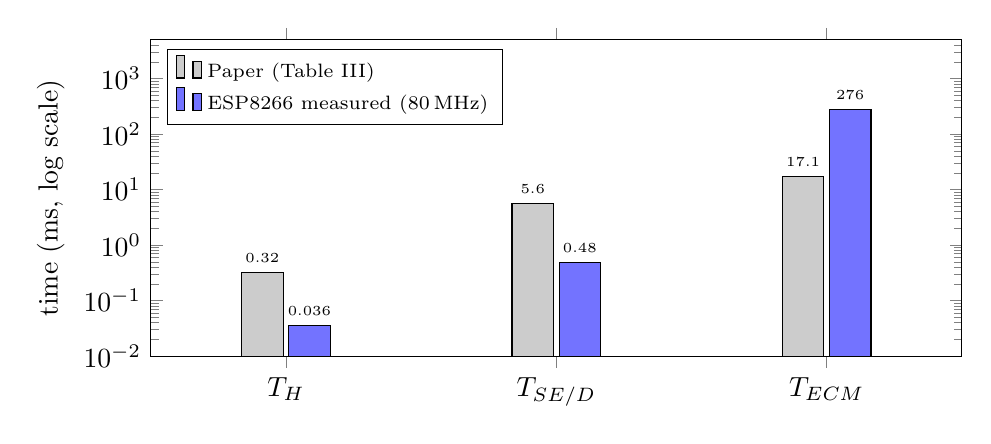
\begin{tikzpicture}
\begin{axis}[
  ybar, ymode=log, log origin=infty, width=0.98\columnwidth, height=5.6cm, bar width=15pt,
  ymin=0.01, ymax=5000, ylabel={time (ms, log scale)},
  symbolic x coords={$T_H$,$T_{SE/D}$,$T_{ECM}$},
  xtick=data, legend style={at={(0.02,0.97)},anchor=north west,font=\scriptsize,cells={anchor=west}},
  point meta=explicit symbolic,
  nodes near coords, nodes near coords style={font=\tiny,anchor=south},
  enlarge x limits=0.25]
\addplot[fill=gray!40] coordinates {($T_H$,0.32) [0.32] ($T_{SE/D}$,5.6) [5.6] ($T_{ECM}$,17.1) [17.1]};
\addplot[fill=blue!55] coordinates {($T_H$,0.0363) [0.036] ($T_{SE/D}$,0.4845) [0.48] ($T_{ECM}$,276.35) [276]};
\legend{Paper (Table III), ESP8266 measured (80\,MHz)}
\end{axis}
\end{tikzpicture}
\caption{Assumed versus measured per-operation time on the ESP8266 ($T_{SE/D}$ is \texttt{aes\_big} GCM; \texttt{aes\_ct} gives 1.15\,ms).}
\label{fig:constants}
\end{figure}

\subsection{Recomputed ranking}
\label{sec:ranking}
\textbf{Against ECC-based schemes} the proposed scheme is far cheaper than the paper states. On the ESP8266 at 80\,MHz (device plus server, AES-GCM, \texttt{aes\_big}/\texttt{aes\_ct}) it costs 2.1/4.7\,ms, whereas Sadhukhan, Shuai and Cheng--Le cost 279--553\,ms, Challa 2\,487\,ms and Poorambage 5\,251\,ms, i.e.\ about 120--3\,000$\times$ more. (Challa and Wazid include the fuzzy-extraction time $T_{fe}$, which we did not measure and keep at the paper's value.)

\textbf{Against the hash-only schemes} (Turkanovic, Dhillon--Karla, Jiang) the outcome depends on whether the session KDF is counted. The proposed scheme beats a hash-only scheme only if $r=T_{SE/D}/T_H$ is below roughly 2.0--4.5, depending on the cost column; the paper's own constants give $r=17.5$. With Table~V as printed (V1), the hash-only schemes are cheaper in all 12 AES-GCM sensitivity cells on the ESP8266 at both clocks ($r=6.7$--31.6, i.e.\ 3.8--10.8$\times$ cheaper), in 11 of 12 on the Graviton2 core, and in 6 of 12 on the laptop. But measured HKDF-SHA256 costs $6$--$17\,T_H$ on every platform, against $5$--$7\,T_H$ for the hash-only device columns, so a device that must run the session KDF already costs more than they do before any encryption. Table~\ref{tab:variants} shows that counting the KDF (V2--V4) makes all three hash-only schemes cheaper than the proposed scheme in every column on every platform we measured, including OpenSSL's hardware AES and SHA (GCM 78\,ns, SHA-1 38\,ns, HKDF 232\,ns per call). The ranking flips only if $T_{SE/D}$ is read as unauthenticated AES (one block or CTR without a MAC), which drops the MAC the scheme requires. The operation-count model also under-predicts the implementation: it gives 2.4\,ms of device compute (\texttt{aes\_ct}) where we measure 5.3\,ms.

\begin{table}[t]
\caption{Number of the three hash-only schemes that cost \emph{less} than the proposed scheme (device$+$server total; GCM with cached key, \texttt{aes\_big}; V1--V4 as defined in Section~\ref{sec:method}).}
\label{tab:variants}
\centering
\small
\begin{tabular}{@{}lcccc@{}}
\toprule
Platform & V1 & V2 & V3 & V4 \\
\midrule
ESP8266, 80 and 160\,MHz (BearSSL) & 3/3 & 3/3 & 3/3 & 3/3 \\
Graviton2 t4g.nano (BearSSL) & 3/3 & 3/3 & 3/3 & 3/3 \\
Laptop, BearSSL software & 3/3 & 3/3 & 3/3 & 3/3 \\
Laptop, OpenSSL hardware AES/SHA & 1/3 & 3/3 & 3/3 & 3/3 \\
\bottomrule
\end{tabular}
\end{table}

\subsection{Protocol-level observations}
\label{sec:protocol}
\textbf{No forward secrecy.} The session key depends on $k^\star$, $N_i$, $N_j$ and $t$ (Eq.~16); $N_i$, $N_j$ and $t$ travel encrypted only under $k^\star$. An attacker who later obtains $k^\star$ recovered all 5 of 5 past session keys from recorded $M_1$/$M_2$ alone. We did not check whether the compared ECC-based schemes provide forward secrecy, so whether the comparison is like for like remains open.

\textbf{ECC is not used online, and is nominal.} Eq.~8 defines $\lambda_X$ as a hash reduced modulo $n$, not a curve operation; the public point $P_X=\lambda_X G$ is set only optionally and Eqs.~9--22 never use it. Every online operation is a hash, KDF, encryption or MAC.

\textbf{Server cost is linear in the number of devices.} Because $\mathrm{PID}=H_2(\lambda\,\|\,t)$ is unlinkable, the server cannot index by pseudonym and must probe (devices $\times$ epoch window). On the laptop one resolution took 4.8\,ms at 1\,000 and 23.9\,ms at 5\,000 devices (a 13-epoch window), against the constant server cost of Table~V. A precomputed table avoids the compute but needs $1\,000\times25\times32$\,B $=800$\,KB at 1\,000 devices against the paper's 320-bit server storage (Table~VI): either way the scheme pays $O(N\cdot W)$.

\section{Discussion and Threats to Validity}
The paper's advantage over ECC-based schemes is real and larger than reported, but those schemes may provide different properties. Its claimed processing advantage over hash-only schemes is not supported once the session KDF that its own equations require is counted; it appears only when that step is omitted and AES-GCM is unusually cheap relative to SHA-1. Its communication and storage claims cannot be checked, because the paper's tables and text disagree.

\textbf{Threats to validity.} We measured one microcontroller class (32-bit); the paper's targets include 8- and 16-bit parts, and we did not measure an MCU with AES or SHA hardware or energy. Primitive costs are BearSSL's and OpenSSL's; other libraries shift constants, although the KDF result depends on HKDF costing several hash operations, not on absolute speed. A hardware HKDF/HMAC engine could change it. Competitor costs use the operation counts of~\cite{base}, which we did not verify against the original papers; $T_C$ and $T_{fe}$ were not measured. The elliptic-curve benchmark ran on a temporary heap stack on the ESP8266 (the 4\,KB task stack is too small), with outputs verified by checksum. The t4g.nano is a shared-host cloud VM pinned to one core, so its absolute numbers are indicative only, and it has no hardware-crypto measurement. Figure values were read by eye. Our implementation is one reading of a specification that leaves the epoch and replay window undefined (it is held in RAM in the Python reference; the firmware persists it to flash).

\section{Conclusion and Future Work}
Measured on real hardware, the protocol's cost model is dominated by two things the paper's constants get wrong: an ECC scalar multiplication on a small MCU is sixteen times slower than assumed, and the session-key derivation is several times more expensive than a hash. The first makes the scheme look better against ECC-based schemes than the paper claims; the second makes it look worse against hash-only schemes. The paper's stated percentages cannot be reproduced from its own data. Future work: measure an MCU with hardware AES and SHA and a Raspberry Pi~3; verify the competitors' operation counts and security properties against their original papers; contact the authors about the derivation of the headline percentages; and complete the TA-assisted key-revocation extension we proposed earlier, which none of the compared schemes specify.

\section*{Reproducibility}
The Python reference implementation, the C device core, the ESP8266 firmware and benchmark, the audit scripts and all raw data (including output checksums) are in the project repository \texttt{[REPO-URL]} under \texttt{firmware/esp8266/} and \texttt{research/paper\_audit/}; \texttt{FINDINGS.md} lists the commands.

\begin{thebibliography}{99}
\bibitem{base} A. Al-Rasheed, R. Khan, A. Ahmad, A. Saeed, F. Alturise, and S. Alkhalaf, ``A low-cost hybrid elliptic curve cryptography authentication protocol for trustworthy Internet of Things communication,'' \emph{IEEE Trans. Consum. Electron.}, vol.~72, no.~2, pp.~4483--4491, May 2026.
\bibitem{porambage} P. Porambage, C. Schmitt, P. Kumar, A. Gurtov, and M. Ylianttila, ``Two-phase authentication protocol for wireless sensor networks in distributed IoT applications,'' in \emph{Proc. IEEE Wireless Commun. Netw. Conf. (WCNC)}, Apr. 2014, pp.~2728--2733.
\bibitem{turkanovic} M. Turkanovi\'c, B. Brumen, and M. H\"olbl, ``A novel user authentication and key agreement scheme for heterogeneous ad hoc wireless sensor networks, based on the Internet of Things notion,'' \emph{Ad Hoc Netw.}, vol.~20, pp.~96--112, Sep. 2014.
\bibitem{dhillon} P. K. Dhillon and S. Kalra, ``A lightweight biometrics based remote user authentication scheme for IoT services,'' \emph{J. Inf. Secur. Appl.}, vol.~34, pp.~255--270, Jun. 2017.
\bibitem{jiang} Q. Jiang, F. Wei, S. Fu, J. Ma, G. Li, and A. Alelaiwi, ``Robust extended chaotic maps-based three-factor authentication scheme preserving biometric template privacy,'' \emph{Nonlinear Dyn.}, vol.~83, no.~4, pp.~2085--2101, Mar. 2016.
\bibitem{challa} S. Challa \emph{et al.}, ``Secure signature-based authenticated key establishment scheme for future IoT applications,'' \emph{IEEE Access}, vol.~5, pp.~3028--3043, 2017.
\bibitem{sadhukhan} D. Sadhukhan, S. Ray, G. P. Biswas, M. K. Khan, and M. Dasgupta, ``A lightweight remote user authentication scheme for IoT communication using elliptic curve cryptography,'' \emph{J. Supercomput.}, vol.~77, no.~2, pp.~1114--1151, Feb. 2021.
\bibitem{fakroon} M. Fakroon, M. Alshahrani, F. Gebali, and I. Traore, ``Secure remote anonymous user authentication scheme for smart home environment,'' \emph{Internet of Things}, vol.~9, Art.~no.~100158, Mar. 2020.
\bibitem{bearssl} T. Pornin, ``BearSSL, a smaller SSL/TLS library,'' \url{https://bearssl.org}. The ESP8266 Arduino core ships a port of BearSSL.
\bibitem{openssl} OpenSSL Project, ``OpenSSL cryptography and SSL/TLS toolkit,'' \url{https://www.openssl.org}.
\bibitem{hkdf} H. Krawczyk and P. Eronen, ``HMAC-based extract-and-expand key derivation function (HKDF),'' RFC 5869, May 2010.
\bibitem{gcm} M. Dworkin, ``Recommendation for block cipher modes of operation: Galois/Counter Mode (GCM) and GMAC,'' NIST SP 800-38D, Nov. 2007.
\end{thebibliography}

\end{document}
